%%%%%%%%%%%%%%%%%%%%%%%%%%%%%%%%%%%%%%%%%%%%%%%%%%%%%%%%%%%%%%%%%%%%%%
% How to use writeLaTeX: 
%
% You edit the source code here on the left, and the preview on the
% right shows you the result within a few seconds.
%
% Bookmark this page and share the URL with your co-authors. They can
% edit at the same time!
%
% You can upload figures, bibliographies, custom classes and
% styles using the files menu.
%
%%%%%%%%%%%%%%%%%%%%%%%%%%%%%%%%%%%%%%%%%%%%%%%%%%%%%%%%%%%%%%%%%%%%%%

\documentclass[12pt]{article}

\usepackage{sbc-template}

\usepackage{graphicx,url}

\usepackage[brazilian]{babel}   
\usepackage[T1]{fontenc} % Codificação para fontes com suporte a caracteres acentuados
\usepackage[utf8]{inputenc} % Codificação UTF-8 (necessário apenas para pdflatex)
\usepackage{multicol}
\usepackage{multirow}
\usepackage{graphicx,url}
\usepackage{amsmath,amssymb,amsfonts}
\usepackage{algorithmic}
\usepackage{textcomp}
\usepackage{url}
\usepackage{enumerate}
\usepackage{multirow}
\usepackage{soul}
\usepackage{verbatim}
\usepackage[table,xcdraw]{xcolor}
\usepackage[shortlabels]{enumitem}
\usepackage{scalefnt} % pacote para diminuir fonte das tabelas
\usepackage{comment} % pacote de comentarios
\usepackage{lscape}
\usepackage{fancyhdr}
\usepackage{IHC}
\usepackage[super]{nth}
\usepackage{pdfcomment} %By IHC 2026: package to insert description in images | pacote para inserir descrição nas imagens

%previne hifenização
\tolerance=1
\emergencystretch=\maxdimen
\hyphenpenalty=10000
\hbadness=10000

\sloppy

\input{IHC_info}

\title{A Web-Based Educational Game to Support the Understanding of
Nielsen's Heuristics Through Paired Scenarios: An Experience Report}

% Authors and affiliations omitted for double-blind review (IHC 2026).
% Reinstate in the camera-ready version, along with the CAAE number in the
% "Cuidados Éticos" section.
\author{Authors omitted for double-blind review}

\address{Affiliations omitted for double-blind review
  \email{Emails omitted for double-blind review}
}

\begin{document} 

%%  ATENÇÃO: AS INFORMAÇÕES DESTACADAS EM AZUL SÃO APENAS PARA INFORMAR OS AJUSTES NO TEMPLATE DA SBC E ACRESCENTAR INSTRUÇÕES DE ACESSIBILIDADE. O SEU TEXTO NÃO DEVE ESTAR NA COR AZUL.

\maketitle

\thispagestyle{plain}

% Structured abstract (ABNT 6028:2021 adaptation) -- max 10 lines.
\begin{abstract}
\textbf{Introduction}: Teaching Nielsen's usability heuristics traditionally relies on reading abstract definitions, which novices often find hard to internalize.
\textbf{Objective}: To support the teaching of Nielsen's heuristics through paired interactive scenarios.
\textbf{Methodology}: Design and evaluation of a web-based educational game where players complete each task in paired violating and compliant interfaces, with narration and gamification; open-ended responses were analysed via qualitative content analysis.
\textbf{Results}: Initial results suggest the paired bad/good contrast is the main mechanism supporting learning over traditional reading; narration served as a focusing aid, gamification as mild engagement scaffolding rather than a learning driver.
\end{abstract}

\keywords{Nielsen's usability heuristics, HCI education, educational game, game-based learning, experience report.}

% Per IHC 2026 rules, a Portuguese "resumo" / "palavras-chave" block is required
% only for papers written in Portuguese. This paper is in English, so the
% resumo and palavraschave blocks are intentionally omitted.

\section{General Information}

All full papers and posters (short papers) submitted to some SBC conference,
including any supporting documents, should be written in English or in
Portuguese. The format paper should be A4 with single column, 3.5 cm for upper
margin, 2.5 cm for bottom margin and 3.0 cm for lateral margins, without
headers or footers. The main font must be Times, 12 point nominal size, with 6
points of space before each paragraph. Page numbers must be suppressed.

Full papers must respect the page limits defined by the conference.
Conferences that publish just abstracts ask for \textbf{one}-page texts.

\section{First Page} \label{sec:firstpage}

The first page must display the paper title, the name and address of the
authors, the abstract in English and ``resumo'' in Portuguese (``resumos'' are
required only for papers written in Portuguese). The title must be centered
over the whole page, in 16 point boldface font and with 12 points of space
before itself. Author names must be centered in 12 point font, bold, all of
them disposed in the same line, separated by commas and with 12 points of
space after the title. Addresses must be centered in 12 point font, also with
12 points of space after the authors' names. E-mail addresses should be
written using font Courier New, 10 point nominal size, with 6 points of space
before and 6 points of space after.

The abstract and ``resumo'' (if is the case) must be in 12 point Times font,
indented 0.8cm on both sides. The word \textbf{Abstract} and \textbf{Resumo},
should be written in boldface and must precede the text.

\section{CD-ROMs and Printed Proceedings}

In some conferences, the papers are published on CD-ROM while only the
abstract is published in the printed Proceedings. In this case, authors are
invited to prepare two final versions of the paper. One, complete, to be
published on the CD and the other, containing only the first page, with
abstract and ``resumo'' (for papers in Portuguese).

\section{Sections and Paragraphs}

Section titles must be in boldface, 13pt, flush left. There should be an extra
12 pt of space before each title. Section numbering is optional. The first
paragraph of each section should not be indented, while the first lines of
subsequent paragraphs should be indented by 1.27 cm.

\subsection{Subsections}

The subsection titles must be in boldface, 12pt, flush left. 

\section{Figures and Captions}\label{sec:figs}


Figure and table captions should be centered if less than one line
(Figure~\ref{fig:exampleFig1}), otherwise justified and indented by 0.8cm on
both margins, as shown in Figure~\ref{fig:exampleFig2}. The caption font must
be Helvetica, 10 point, boldface, with 6 points of space before and after each
caption.

\begin{figure}[ht]
\centering
% By IHC 2026: \pdftooltip used to make the image description readable by screen readers. Used with the \usepackage{pdfcomment} package
%\pdftooltip usado para definir a descrição da imagem a ser lida por leitores de tela. Usado com o pacote \usepackage{pdfcomment} 
 \pdftooltip{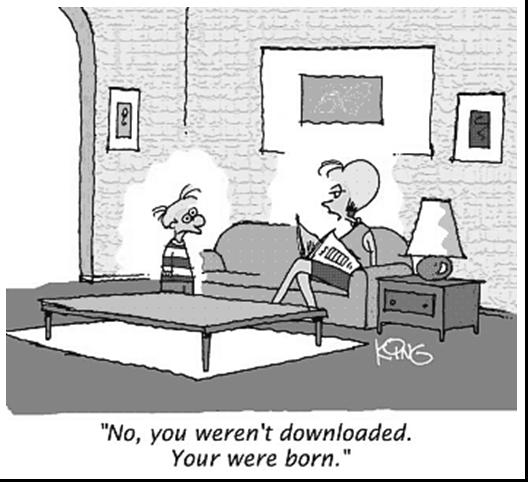
\includegraphics[width=.5\textwidth]{Figuras/fig1.jpg}}
 %By IHC 2026: image description between {} / descrição da imagem entre {}
{The image is a black-and-white cartoon showing a living room where a woman sits on a sofa reading a magazine, while a child stands watching her. The woman responds to the child by saying, "No, you weren't downloaded. You were born." The scene is humorous, contrasting the technological concept of "downloading" with the natural process of birth, suggesting that the child, immersed in the digital world, confuses the two.}
\caption{A typical figure.}
\label{fig:exampleFig1}
\end{figure}



\begin{figure}[ht]
\centering
 \pdftooltip{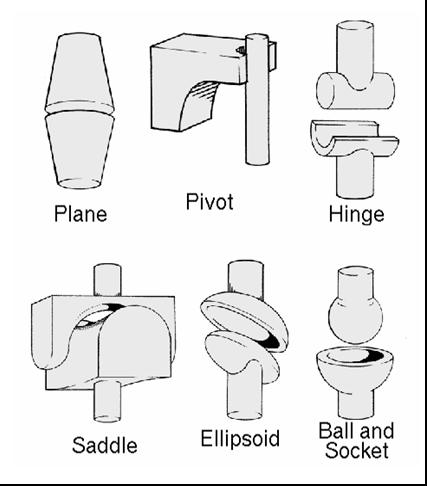
\includegraphics[width=.3\textwidth]{Figuras/fig2.jpg}}
{The image shows six types of synovial joints in the human body, each illustrated with a schematic drawing. They are: plane joint, which allows gliding movements; pivot joint, which allows rotation around an axis; hinge joint, similar to a door, allowing flexion and extension; saddle joint, which allows movement in two directions; ellipsoid joint, with mobility in several axes; and ball-and-socket joint, which offers wide freedom of movement in several directions.}
\caption{This figure is an example of a figure caption taking more than one
  line and justified considering margins mentioned in Section~\ref{sec:figs}.}
\label{fig:exampleFig2}
\end{figure}



\section{Tables}

In tables, try to avoid the use of colored or shaded backgrounds, and avoid
thick, doubled, or unnecessary framing lines. When reporting empirical data,
do not use more decimal digits than warranted by their precision and
reproducibility. \textcolor{blue}{Table caption must be placed before the table (see Table 1)}
and the font used must also be Helvetica, 10 point, boldface, with 6 points of
space before and after each caption. \textcolor{blue}{Note: Table has no side borders.}

\begin{table}
  \caption{Frequency of Special Characters.}
  \centering
  \label{tab:freq}
  \begin{tabular}{c|c|l}
    \hline
    Non-English or Math&Frequency&Comments\\
    \hline
    \O & 1 in 1,000& For Swedish names\\
    \hline
    $\pi$ & 1 in 5& Common in math\\
    \hline
    \$ & 4 in 5 & Used in business\\
    \hline
    $\Psi^2_1$ & 1 in 40,000& Unexplained usage\\
    \hline
\end{tabular}
\end{table}
\subsection{Creating accessible tables}

\textcolor{blue}{This content was prepared especially for authors submitting papers to the IHC 2026 event. More details are available at: \url{https://ihc.sbc.org.br/2026/en/resources/}.}

\begin{itemize}
    \item \textbf{Clearly label clear column and row headers:} Make sure each column and row has clear, descriptive headers. This helps users understand what each piece of data represents. Mark these headers correctly in the table properties if you use software that allows this (such as HTML, Word, or LaTeX);
    \item \textbf{Keep a simple structure:} Avoid overly complicated tables, such as nested tables, tables with multiple layers of headers, or many rows and columns. Consider splitting complex data into multiple smaller tables if necessary;
    \item \textbf{Avoid leaving empty cells:} Empty cells can confuse when reading the document. If a cell is intentionally empty, consider adding explanatory text, such as "N/A" (not applicable) or "0", as appropriate;
    \item \textbf{Use adequate color contrast:} Ensure that the text and table backgrounds have enough contrast to be easily readable by everyone, including people with low vision or difficulty distinguishing some colors;
    \item \textbf{Provide a description or summary:} Include a brief summary or description of the table, highlighting key findings, trends, or important points. This provides context that helps screen reader users understand what to look for in the table;
    \item \textbf{Properly label units of measurement:} If your data includes units of measurement, make sure they are clearly stated and consistent throughout the table.
\end{itemize}

\begin{comment}
    Em português
    \subsection{Criando tabelas acessíveis}
    
    Este conteúdo foi preparado especialmente para autores que submeterão artigos para o evento IHC 2026. Mais detalhes estão disponíveis em: \url{https://ihc.sbc.org.br/2026/index.php/recursos/}.
    
    \begin{itemize}
    \item \textbf{Identifique claramente os cabeçalhos de colunas e linhas:} Certifique-se de que cada coluna e linha tenha cabeçalhos claros e descritivos. Isso ajuda os usuários a entender o que cada dado representa. Marque esses cabeçalhos corretamente nas propriedades da tabela se você usar um software que permita isso (como HTML, Word ou LaTeX);
    \item \textbf{Mantenha uma estrutura simples:} Evite tabelas muito complexas, como tabelas aninhadas, tabelas com várias camadas de cabeçalhos ou muitas linhas e colunas. Considere dividir dados complexos em várias tabelas menores, se necessário;
    \item \textbf{Evite deixar células vazias:} Células vazias podem confundir a leitura do documento. Se uma célula estiver intencionalmente vazia, considere adicionar um texto explicativo, como "N/A" (Não Aplicável) ou "0", conforme apropriado;
    \item \textbf{Use contraste de cores adequado:} Certifique-se de que o texto e o fundo da tabela tenham contraste suficiente para serem facilmente legíveis por todos, incluindo pessoas com baixa visão ou dificuldade em distinguir algumas cores;
    \item \textbf{Forneça uma descrição ou resumo:} Inclua um breve resumo ou descrição da tabela, destacando as principais descobertas, tendências ou pontos importantes. Isso fornece contexto que ajuda os usuários de leitores de tela a entender o que procurar na tabela;
    \item \textbf{Rotule corretamente as unidades de medida:} Se os seus dados incluírem unidades de medida, certifique-se de que elas estejam claramente indicadas e sejam consistentes em toda a tabela.
    \end{itemize}
\end{comment}


\section{Images}

All images and illustrations should be in black-and-white, or gray tones,
excepting for the papers that will be electronically available (on CD-ROMs,
internet, etc.). The image resolution on paper should be about 600 dpi for
black-and-white images, and 150-300 dpi for grayscale images.  Do not include
images with excessive resolution, as they may take hours to print, without any
visible difference in the result. 

\subsection{Figure Description}

\textcolor{blue}{This content was prepared especially for authors submitting papers to the IHC 2026 event. More details are available at: \url{https://ihc.sbc.org.br/2026/en/resources/}.}

 \textcolor{blue}{The goal of image descriptions for screen reader users is to provide a similar experience to users who can view the images. By following these tips, you can create more useful and accessible descriptions.}

\begin{itemize}
    \item \textbf{Be clear and concise:} Use simple and objective language. Describe the image clearly and directly, without using long or complicated sentences;
    \item \textbf{Be descriptive:} Include important details contributing to understanding the image. This can include colors, shapes, facial expressions, actions, and context. Try to convey the same information that a person viewing the image would receive;
    \item \textbf{Orient the position of the elements:} It is recommended to describe the elements from top to bottom, left to right unless the photograph's focus is elsewhere. Remember that the point of view must always be that of the person observing the photo to indicate the positioning (left, right);
    \item \textbf{Focus on the essential:} Identify the image's most important element and start there. It is not necessary to describe every detail but rather the most significant aspects related to the text's content or the image's purpose;
    \item \textbf{Avoid saying "image of" or "photo of":} Go straight to the description. Screen readers usually already announce that it is an image, so this information is redundant;
    \item \textbf{Be sensitive to context:} The description must be in harmony with the content of the surrounding text. For example, if an image has a specific purpose in an article or post, the description should reflect that purpose;
    \item \textbf{Avoid subjective interpretations:} Describe what you see, not what you think or feel about the image. Avoid using language that could be interpreted differently by different people;
    \item \textbf{Don't ignore text embedded in images:} If text is inside an image, transcribe that text in the description. This is especially important for buttons, banners, and informational graphics;
    \item \textbf{Test accessibility:} After adding image descriptions, it is a good practice to test accessibility using screen readers to ensure the descriptions are effective. A free suggestion is the NVDA tool, available at the link: \url{https://www.nvaccess.org/download/}.
    
 %In latex, use the \usepackage{pdfcomment} package and in the figure use \pdftooltip{}. See example in the images above.
\end{itemize}

\begin{comment}
    Em português
    \subsection{Descrição de Figura}
    
    Este conteúdo foi preparado especialmente para autores que submeterão artigos para o evento IHC 2026. Mais detalhes estão disponíveis em: \url{https://ihc.sbc.org.br/2026/index.php/recursos/}.
    
    O objetivo das descrições de imagens para usuários de leitores de tela é proporcionar uma experiência semelhante aos usuários que podem visualizá-las. Seguindo estas dicas, você pode criar descrições mais úteis e acessíveis.
    
    \begin{itemize}
    \item \textbf{Seja claro e conciso:} Use uma linguagem simples e objetiva. Descreva a imagem de forma clara e direta, sem usar frases longas ou complicadas;
    \item \textbf{Seja descritivo:} Inclua detalhes importantes que contribuam para a compreensão da imagem. Isso pode incluir cores, formas, expressões faciais, ações e contexto. Tente transmitir as mesmas informações que uma pessoa visualizando a imagem receberia;
    \item \textbf{Oriente a posição dos elementos:} Recomenda-se descrever os elementos de cima para baixo, da esquerda para a direita, a menos que o foco da fotografia esteja em outro lugar. Lembre-se de que o ponto de vista deve ser sempre o de quem observa a foto para indicar o posicionamento (esquerda, direita);
    \item \textbf{Concentre-se no essencial:} Identifique o elemento mais importante da imagem e comece por ele. Não é necessário descrever todos os detalhes, mas sim os aspectos mais significativos relacionados ao conteúdo do texto ou à finalidade da imagem;
    \item \textbf{Evite dizer "imagem de" ou "foto de":} Vá direto para a descrição. Leitores de tela geralmente já anunciam que se trata de uma imagem, portanto, essa informação é redundante;
    \item \textbf{Seja sensível ao contexto:} A descrição deve estar em harmonia com o conteúdo do texto ao redor. Por exemplo, se uma imagem tem uma finalidade específica em um artigo ou publicação, a descrição deve refletir essa finalidade;
    \item \textbf{Evite interpretações subjetivas:} Descreva o que você vê, não o que você pensa ou sente sobre a imagem. Evite usar linguagem que possa ser interpretada de forma diferente por pessoas diferentes;
    \item \textbf{Não ignore o texto incorporado em imagens:} Se o texto estiver dentro de uma imagem, transcreva-o na descrição. Isso é especialmente importante para botões, banners e gráficos informativos;
    \item \textbf{Teste a acessibilidade:} Após adicionar as descrições das imagens, é uma boa prática testar a acessibilidade usando leitores de tela para garantir que as descrições sejam eficazes. Uma sugestão gratuita é a ferramenta NVDA, disponível no link: \url{https://www.nvaccess.org/download/}.
    \end{itemize}
    
    No latex, use o pacote \usepackage{pdfcomment} e na figura use \pdftooltip{}. Ver exemplo nas imagens acima.

\end{comment}

\subsection{Graph description}  

\textcolor{blue}{This content was also prepared especially for authors submitting papers to the IHC 2026 event. More details are available at: \url{https://ihc.sbc.org.br/2026/en/resources/}.}

 \textcolor{blue}{Creating effective graph descriptions for screen reader users ensures everyone can access the same information.}

\begin{itemize}
  \item \textbf{Describe the purpose of the graph:} Start by explaining what the graph is trying to show or what question it is trying to answer. This gives the user a clear understanding of the context before entering the details;
    \item \textbf{Explain the type of graph:} Indicate whether it is a bar graph, line graph, pie graph, etc. This helps the user form a mental image of the arrangement of the data;
    \item \textbf{Describe the axes:} For line or bar charts, describe the axes, including what they represent and any units of measurement. Enter the minimum and maximum values and the scale if relevant;
    \item \textbf{Highlight key trends or patterns:} Instead of listing all the data, focus on key trends, spikes, dips, or notable patterns. For example, "The graph shows a steady increase in sales from 2010 to 2015.";
    \item \textbf{Use clear, descriptive comparisons:} Instead of saying "huge increase," you can say, "the graph shows a threefold increase in sales between January and February.";
    \item \textbf{Provide a summary or conclusion:} End with a brief summary or conclusion that users can draw from the chart;
    \item \textbf{Use descriptive captions and titles:} Captions and titles should be informative and complement the alternative text you provide;
    \item \textbf{Test accessibility:} After adding your chart descriptions, it is a good practice to test accessibility using screen readers to ensure the descriptions are effective. A free suggestion is the NVDA tool, available at the link: \url{https://www.nvaccess.org/download/}.
\end{itemize}

\begin{comment}
    Em português
    
    \subsection{Descrição de gráfico}
    
    Este conteúdo também foi preparado especialmente para autores que submeterão artigos para o evento IHC 2026. Mais detalhes estão disponíveis em: \url{https://ihc.sbc.org.br/2026/index.php/recursos/}.
    
    Criar descrições de gráficos eficazes para usuários de leitores de tela garante que todos possam acessar as mesmas informações.
    
    \begin{itemize}
    \item \textbf{Descreva a finalidade do gráfico:} Comece explicando o que o gráfico está tentando mostrar ou qual pergunta ele está tentando responder. Isso dá ao usuário uma compreensão clara do contexto antes de inserir os detalhes;
    \item \textbf{Explique o tipo de gráfico:} Indique se é um gráfico de barras, de linhas, de pizza, etc. Isso ajuda o usuário a formar uma imagem mental da disposição dos dados;
    \item \textbf{Descreva os eixos:} Para gráficos de linhas ou barras, descreva os eixos, incluindo o que eles representam e as unidades de medida. Insira os valores mínimo e máximo e a escala, se relevante;
    \item \textbf{Destaque as principais tendências ou padrões:} Em vez de listar todos os dados, se concentre nas principais tendências, picos, quedas ou padrões notáveis. Por exemplo, "O gráfico mostra um aumento constante nas vendas de 2010 a 2015.";
    \item \textbf{Use comparações claras e descritivas:} Em vez de dizer "aumento enorme", você pode dizer "o gráfico mostra um aumento triplicado nas vendas entre janeiro e fevereiro.";
    \item \textbf{Forneça um resumo ou conclusão:} Termine com um breve resumo ou conclusão que os usuários possam extrair do gráfico;
    \item \textbf{Use legendas e títulos descritivos:} As legendas e os títulos devem ser informativos e complementar o texto alternativo fornecido;
    \item \textbf{Teste de acessibilidade:} Após adicionar as descrições do seu gráfico, é uma boa prática testar a acessibilidade usando leitores de tela para garantir que as descrições sejam eficazes. Uma sugestão gratuita é a ferramenta NVDA, disponível no link: \url{https://www.nvaccess.org/download/}.
    \end{itemize}
\end{comment}

\section{References}

Bibliographic references must be unambiguous and uniform.  We recommend giving
the author names references in brackets, e.g. \cite{knuth:84},
\cite{boulic:91}, and \cite{smith:99}.

The references must be listed using 12 point font size, with 6 points of space
before each reference. The first line of each reference should not be
indented, while the subsequent should be indented by 0.5 cm.

\bibliographystyle{sbc}
\bibliography{Referencias/referencias}

\end{document}
